\documentclass[runningheads,a4paper,11pt]{report}

\usepackage{algorithmic}
\usepackage{algorithm} 
\usepackage{array}
\usepackage{amsmath}
\usepackage{amsfonts}
\usepackage{amssymb}
\usepackage{amsthm}
\usepackage{caption}
\usepackage{comment} 
\usepackage{epsfig} 
\usepackage{fancyhdr}
\usepackage[T1]{fontenc}
\usepackage{geometry} 
\usepackage{graphicx}
\usepackage[colorlinks]{hyperref} 
\usepackage[latin1]{inputenc}
\usepackage{multicol}
\usepackage{multirow} 
\usepackage{rotating}
\usepackage{setspace}
\usepackage{subfigure}
\usepackage{url}
\usepackage{float}
\usepackage{verbatim}
\usepackage{xcolor}


\geometry{a4paper,top=3cm,left=2.5cm,right=2cm,bottom=2cm}

\renewcommand{\headrulewidth}{2pt}
\renewcommand{\footrulewidth}{2pt}
\renewcommand{\headrule}{\hbox to\headwidth{%
  \color{lime}\leaders\hrule height \headrulewidth\hfill}}
\renewcommand{\footrule}{\hbox to\headwidth{%
  \color{lime}\leaders\hrule height \footrulewidth\hfill}}

\hypersetup{
pdftitle={artTitle},
pdfauthor={name},
pdfkeywords={pdf, latex, tex, ps2pdf, dvipdfm, pdflatex},
bookmarksnumbered,
pdfstartview={FitH},
urlcolor=cyan,
colorlinks=true,
linkcolor=lightblue,
citecolor=cyan,
}
% \pagestyle{plain}

\setcounter{secnumdepth}{3}
\setcounter{tocdepth}{3}

\linespread{1}

% \pagestyle{myheadings}

\makeindex

\begin{document}

\begin{titlepage}
\sloppy

\begin{center}
BABE\c S BOLYAI UNIVERSITY, CLUJ NAPOCA, ROM\^ ANIA

FACULTY OF MATHEMATICS AND COMPUTER SCIENCE

\vspace{5cm}

\Huge \textbf{Early Discovery of Anxiety/Depression in Teenagers Using Digital Tools}

\vspace{1cm}

\normalsize -- MIRPR report --

\end{center}


\vspace{5cm}

\begin{flushright}
\Large{\textbf{Toth Alexandra-Melania \\ Vl\u{a}d\u{a}u Andra-Ioana \\ Mihalcea Ioan-Alexandu}}\\
\textbf {Emails: }
alexandra.melania.toth@stud.ubbcluj.ro, 
andra.vladau@stud.ubbcluj.ro, 
ioan.mihalcea@stud.ubbcluj.ro\\
\textbf{ Specialisation:} Computer Science Romanian
\end{flushright}

\vspace{2cm}

\begin{center}
2024-2025
\end{center}

\end{titlepage}

\pagenumbering{gobble}

\tableofcontents

\newpage

\listoffigures

\newpage



\newpage

\pagenumbering{arabic}


\chapter{Introduction}
\label{chapter:introduction}


\section{Objective:}
\label{section:objective}
Anxiety/Depression for teenagers - To enhance mental health support for teenagers by developing digital tools that can proactively identify signs of anxiety and depression. These tools aim to engage adolescents in their digital environments, whether through chatbots, social media, video games, or other innovative platforms, to provide early intervention and emotional support.


\section{Main Idea:}
\label{section:idea}
The Early Discovery of Anxiety/Depression in Teenagers solution uses digital platforms to identify and monitor mental health challenges among adolescents. The system combines multiple approaches, including AI-powered chatbots capable of conversational analysis, sentiment evaluation through social media interactions, and mental health assessments embedded in video game experiences. By engaging teenagers where they spend most of their time, be it online or in games, the system aims to provide real-time insights and early warnings of anxiety or depression. This integrated solution offers a holistic approach, blending digital engagement with predictive analytics and personalized intervention strategies.

\section{Motivation:}
\label{section:motivation}
Teen anxiety and depression are pressing issues, often going unnoticed due to social stigma, lack of awareness, or teens' reluctance to seek help. Traditional detection methods are limited in reach and timing, missing critical opportunities for early intervention. By embedding intelligent algorithms in digital spaces where teens naturally engage, like social media, chat apps, and video games, we can monitor signs of mental distress in real time.

AI-powered tools, especially those using natural language processing and machine learning, can analyze behavioural patterns, detect early signs of anxiety or depression, and respond immediately, offering instant, personalized support. These algorithms not only provide proactive intervention, but also reduce barriers to help seek by creating a safe, accessible way for adolescents to explore mental health support in familiar digital environments. This intelligent approach can help prevent more serious issues, offering timely and compassionate care to teens who need it most.


\chapter{The Scientific Problem Addressed}
\label{chapter:scientific}

The prevalence of anxiety and depression among teenagers has reached alarming levels in recent years, with studies indicating a sharp increase in mental health issues within this demographic. According to the World Health Organization (WHO), nearly 10 - 20\% of adolescents worldwide experience mental health conditions, with many cases undiagnosed and untreated. These issues, if unaddressed, can lead to long-term psychological, academic, and social consequences.

A significant challenge in addressing teenage mental health lies in early detection of symptoms. Adolescents often hesitate to seek help due to stigma, lack of awareness, or limited access to traditional healthcare services. Additionally, current diagnostic methods rely heavily on self-reporting or clinical observations, which may not capture the nuanced and early signs of anxiety and depression.

In the digital age, teenagers increasingly interact with technology, spending substantial amounts of time on social media platforms, messaging apps, and video games. These environments often capture behavioral patterns and emotional cues that can serve as indicators of mental health challenges. However, traditional mental health interventions have largely overlooked the potential of these digital spaces to provide proactive and non-intrusive support.

The scientific problem addressed by this project centers on bridging this gap by leveraging advanced digital tools to identify, monitor, and provide early interventions for anxiety and depression. Specifically, the project seeks to answer the following key questions:
\begin{itemize}
    \item How can artificial intelligence and sentiment analysis be utilized to identify early signs of anxiety and depression in teenagers through their digital interactions?
    \item What methods can effectively integrate mental health assessments into engaging and non-invasive digital environments such as video games and chatbots?
    \item How can predictive analytics be used to ensure timely and personalized interventions for at-risk adolescents?
\end{itemize}

By addressing these questions, this project aims to create an innovative, evidence-based approach to teenage mental health care. It leverages the ubiquity of digital platforms to provide scalable, accessible, and proactive solutions to a growing global health challenge.


\chapter{Existing Problem-Solving Methods (Related Work)}
\label{chapter:existing-problem}

\section{Description of the Datasets}
\label{section:description}
This study leverages two publicly available datasets sourced from Kaggle to develop and evaluate the proposed digital tools for the early detection of anxiety and depression in teenagers. These datasets include the *Reddit Mental Health Dataset* \cite{reddit_dataset} and the *Emotion Recognition Dataset* \cite{emotion_dataset}. Below, we provide a detailed description of each dataset and the preprocessing steps undertaken.

\subsection{The Datasets}
\label{section:datasets}

\subsubsection{Reddit Mental Health Dataset}
\label{section:reddit}
The *Reddit Mental Health Dataset* contains posts from Reddit users, labeled based on various mental health conditions. For this project, we focused on two relevant categories: \textit{Anxiety} and \textit{Depression}. The dataset originally includes the following categories:
\begin{itemize}
    \item 0: Stress
    \item 1: Depression
    \item 2: Bipolar Disorder
    \item 3: Personality Disorder
    \item 4: Anxiety
\end{itemize}
For our analysis, only posts labeled as \textit{Depression} and \textit{Anxiety} were retained. The \textit{title} column was removed, and the data was concatenated with the *Emotion Recognition Dataset*. To ensure data consistency, null values were removed, and the dataset was balanced to prevent bias towards the larger class.

\subsubsection{Emotion Recognition Dataset}
\label{section:emotion}
The *Emotion Recognition Dataset* includes text samples labeled with six emotion categories:
\begin{itemize}
    \item 0: Anger
    \item 1: Fear
    \item 2: Joy
    \item 3: Love
    \item 4: Sadness
    \item 5: Surprise
\end{itemize}
The labels were transformed into three broader categories to align with our focus on mental health:
\begin{itemize}
    \item \textbf{Anxiety:} Includes posts labeled as \textit{Fear} and \textit{Surprise}.
    \item \textbf{Depression:} Includes posts labeled as \textit{Sadness} and \textit{Anger}.
    \item \textbf{Normal:} Includes posts labeled as \textit{Joy} and \textit{Love}.
\end{itemize}

The resulting dataset combines information from both sources, providing a diverse set of features for model training and evaluation. Oversampling was applied to the \textit{Normal} class to balance its representation with \textit{Anxiety} and \textit{Depression}.

\subsection{Quantitative Analysis of the Datasets}
\label{section:analysis}

\textbf{Small Dataset:} For initial experiments and prototyping, we created a smaller subset by selecting the first 500 rows from each category (\textit{Anxiety} and \textit{Depression}), resulting in a balanced dataset of 1,000 rows.

\textbf{Large Dataset:} The larger dataset used for final model training and testing contains:
\begin{itemize}
    \item \textbf{Anxiety:} 20,290 rows
    \item \textbf{Depression:} 21,796 rows
\end{itemize}
This dataset provides a robust foundation for training predictive models and evaluating their performance.

\subsection{Related Work and Usage of Datasets}
\label{section:usage}
Both datasets have been used in prior research to analyze mental health and emotional patterns through text. For instance:
\begin{itemize}
    \item The *Reddit Mental Health Dataset* has been utilized to study language patterns associated with mental health conditions and develop classification models for mental health prediction. Studies have achieved notable accuracy in identifying conditions like anxiety and depression using natural language processing (NLP) techniques.
    \item The *Emotion Recognition Dataset* has been widely used for emotion classification tasks, leveraging machine learning models to distinguish between different emotional states.
\end{itemize}

In this project, we extend these works by combining both datasets, re-labeling their categories to focus specifically on anxiety, depression, and normal states, and balancing the data to enhance model performance. By addressing class imbalances and tailoring the datasets to the problem, we aim to improve the detection of mental health conditions in digital interactions.

\subsection{Preprocessing and Data Transformation}
\label{section:preprocessing}
\begin{itemize}
    \item Extracted relevant labels and mapped them to \textit{Depression}, \textit{Anxiety}, and \textit{Normal}.
    \item Removed unnecessary columns such as \textit{title} from the Reddit dataset.
    \item Checked and ensured no null values in the combined dataset.
    \item Performed oversampling on the \textit{Normal} class to address class imbalance.
\end{itemize}

The prepared datasets provide a strong foundation for training advanced AI models capable of identifying early signs of mental health challenges in adolescents.

\vspace{1cm}

\section{First Approach - Small Data}
\label{section:first}

\subsection{Anxiety Data}
\label{section:anxiety}
We used a data set of 500 rows (small data).
\begin{itemize}
    \item \textbf{Hyperparameters:} ID, Text, Target
    \item \textbf{Target:} Normal (246), Anxiety (254)
    \item \textbf{Models:} Support Vector Classification (Support Vector Machine) with encoding Word2Vec
    \item \textbf{Results:}
    \begin{itemize}
        \item \textbf{Accuracy:} 0.64
        \item \textbf{Precision (average):} 0.6481
        \item \textbf{Precision for Anxiety Class:} 0.6481
        \item \textbf{Precision for Normal Class:} 0.6304
        \item \textbf{Recall:} 0.6731
        \item \textbf{Confusion Matrix:}
    \end{itemize}
\end{itemize}

\begin{figure}[H]
\centering
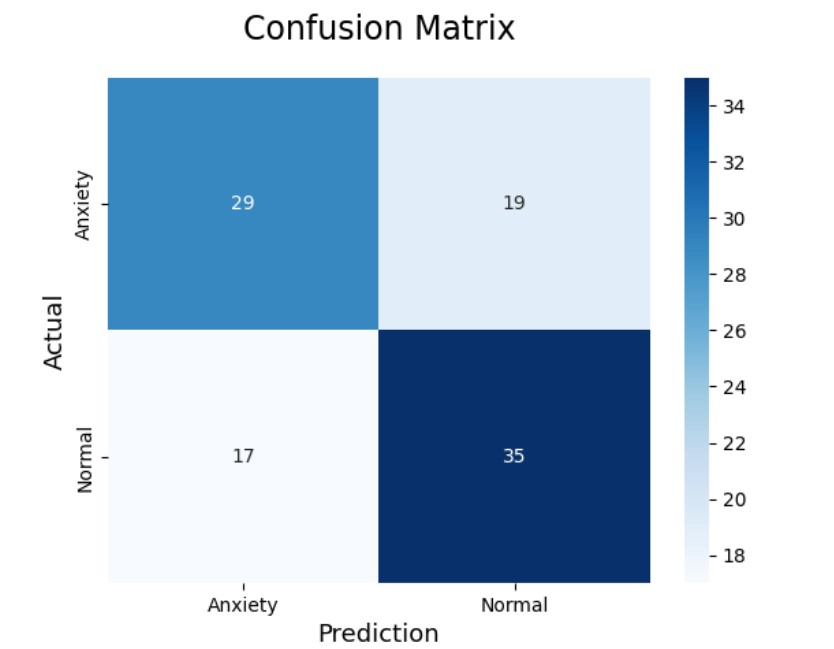
\includegraphics[width=0.9\textwidth]{Anxiety-Data-SmallData.jpg}
\caption[Confusion matrix for anxiety data (small dataset)]{\centering Confusion matrix for anxiety data (small dataset). This matrix shows the classification performance: 29 true positives and 17 false positives for normal cases, and 35 true positives and 19 false negatives for anxiety cases.}
\end{figure}


\vspace{0.5cm} % Add 1 cm of vertical space (adjust as needed)

\subsection{Depression Data}
\label{section:depression}
We used a data set of 500 rows (small data).
\begin{itemize}
    \item \textbf{Hyperparameters:} ID, Text, Target
    \item \textbf{Target:} Normal (249), Depression (251)
    \item \textbf{Models:} Support Vector Classification (Support Vector Machine) with encoding Word2Vec
    \item \textbf{Results:}
    \begin{itemize}
        \item \textbf{Accuracy:} 0.62
        \item \textbf{Precision (average):} 0.6182
        \item \textbf{Precision for Depression Class:} 0.6182
        \item \textbf{Precision for Normal Class:} 0.6222
        \item \textbf{Recall:} 0.6667
        \item \textbf{Confusion Matrix:}
    \end{itemize}
\end{itemize}

\begin{figure}[h]
\centering
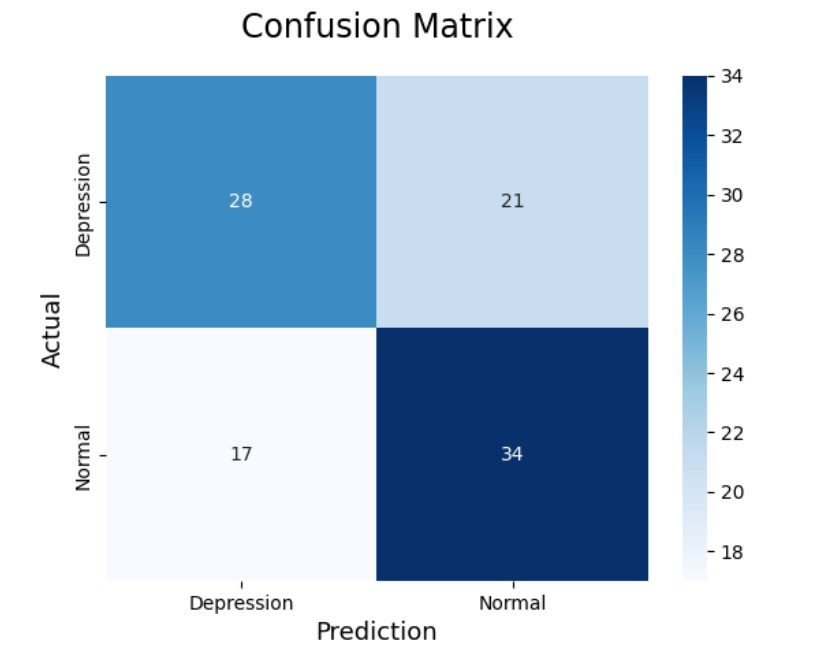
\includegraphics[width=0.9\textwidth]{Depression-Data-SmallData.jpg}
\caption[Confusion matrix for depression data (small dataset)]{\centering Confusion matrix for depression data (small dataset). This matrix illustrates the results with 28 true positives and 17 false positives for normal cases, and 34 true positives and 21 false negatives for depression cases.}
\end{figure}

\vspace{1cm} % Add 1 cm of vertical space (adjust as needed)

\section{Second Approach - Big Data}
\label{section:second}

\subsection{Anxiety Data}
\label{section:anxietydata}

\subsubsection{Linear Regression}
\label{section:linear}

\begin{itemize}
    \item \textbf{Hyperparameters:} ID, Text, Target
    \item \textbf{Target:} Normal (246), Anxiety (254)
    \item \textbf{Models:} Linear Regression with transformer Sentence Transformer with the data set encoding 'all-MiniLM-L6-v2'
    \item \textbf{Results:}
    \begin{itemize}
        \item \textbf{Accuracy:} 0.82
        \item \textbf{Average Precision:} 0.82
        \item \textbf{Precision for Anxiety Class:} 0.82
        \item \textbf{Precision for Normal Class:} 0.82
        \item \textbf{Recall for Anxiety Class:} 0.81
        \item \textbf{Recall for Normal Class:} 0.83
        \item \textbf{Confusion Matrix:}
    \end{itemize}
\end{itemize}

\begin{figure}[h]
\centering
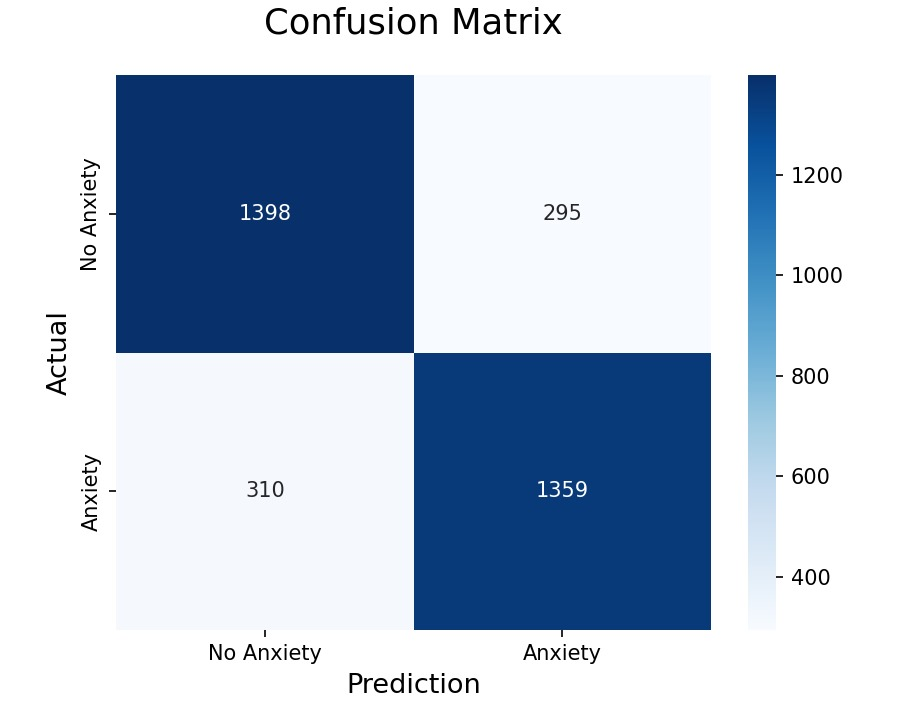
\includegraphics[width=0.9\textwidth]{Anxiety-Data-LinearRegression.jpg}
\caption[Confusion matrix for anxiety data (linear regression)]{\centering Confusion matrix for anxiety data using Linear Regression (large dataset). It details 1398 true positives and 310 false positives for normal cases, along with 1359 true positives and 295 false negatives for anxiety cases.}
\end{figure}

\vspace{1cm} % Add 1 cm of vertical space (adjust as needed)

\subsubsection{Decision Tree}
\label{section:decision}

\begin{itemize}
    \item \textbf{Hyperparameters:} ID, Text, Target
    \item \textbf{Target:} Normal (246), Anxiety (254)
    \item \textbf{Models:} Decision Tree with transformer Sentence Transformer with the data set encoding 'all-MiniLM-L6-v2'
    \item \textbf{Results:}
    \begin{itemize}
        \item \textbf{Accuracy:} 0.83
        \item \textbf{Average Precision:} 0.83
        \item \textbf{Precision for Anxiety Class:} 0.88
        \item \textbf{Precision for Normal Class:} 0.79
        \item \textbf{Recall for Anxiety Class:} 0.75
        \item \textbf{Recall for Normal Class:} 0.90
        \item \textbf{Confusion Matrix:}
    \end{itemize}
\end{itemize}

\begin{figure}[h]
\centering
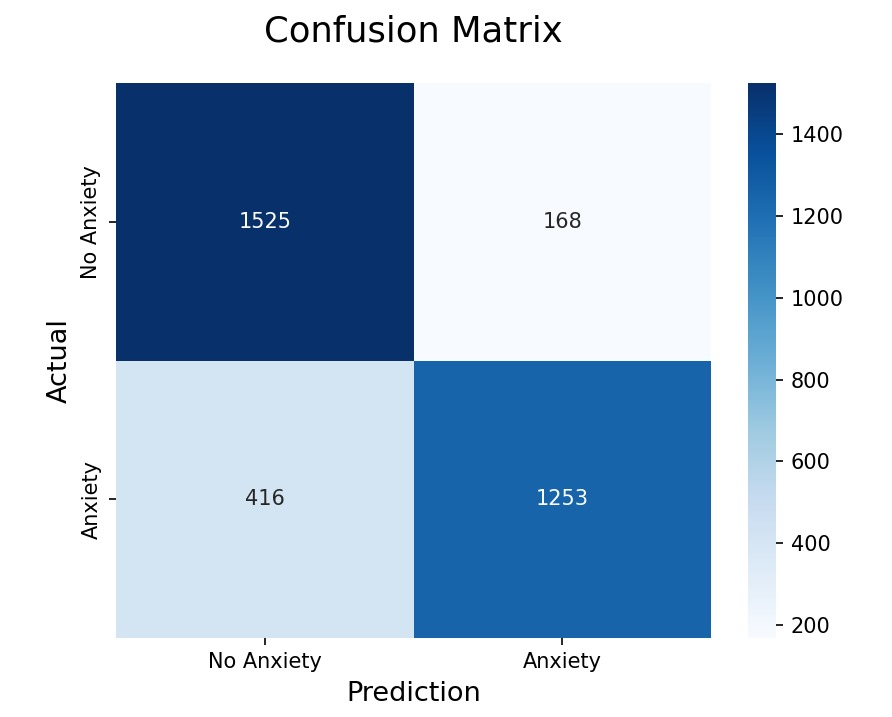
\includegraphics[width=0.9\textwidth]{Anxiety-Data-DecisionTree.jpg}
\caption[Confusion matrix for anxiety data (decision tree)]{\centering Confusion matrix for anxiety data using a Decision Tree (large dataset). The matrix indicates 1525 true positives and 416 false positives for normal cases, with 1253 true positives and 168 false negatives for anxiety cases.}
\end{figure}

\vspace{0.5cm} % Add 1 cm of vertical space (adjust as needed)

\subsubsection{Multi-layer Perceptron Classifier}
\label{section:mpl}

\begin{itemize}
    \item \textbf{Hyperparameters:} ID, Text, Target
    \item \textbf{Target:} Normal (246), Anxiety (254)
    \item \textbf{Models:} Multi-layer Perceptron Classifier with transformer Sentence Transformer with the data set encoding 'all-MiniLM-L6-v2'
    \item \textbf{Results:}
    \begin{itemize}
        \item \textbf{Accuracy:} 0.93
        \item \textbf{Average Precision:} 0.93
        \item \textbf{Precision for Anxiety Class:} 0.95
        \item \textbf{Precision for Normal Class:} 0.90
        \item \textbf{Recall for Anxiety Class:} 0.90
        \item \textbf{Recall for Normal Class:} 0.95
        \item \textbf{Confusion Matrix:}
    \end{itemize}
\end{itemize}

\begin{figure}[h]
\centering
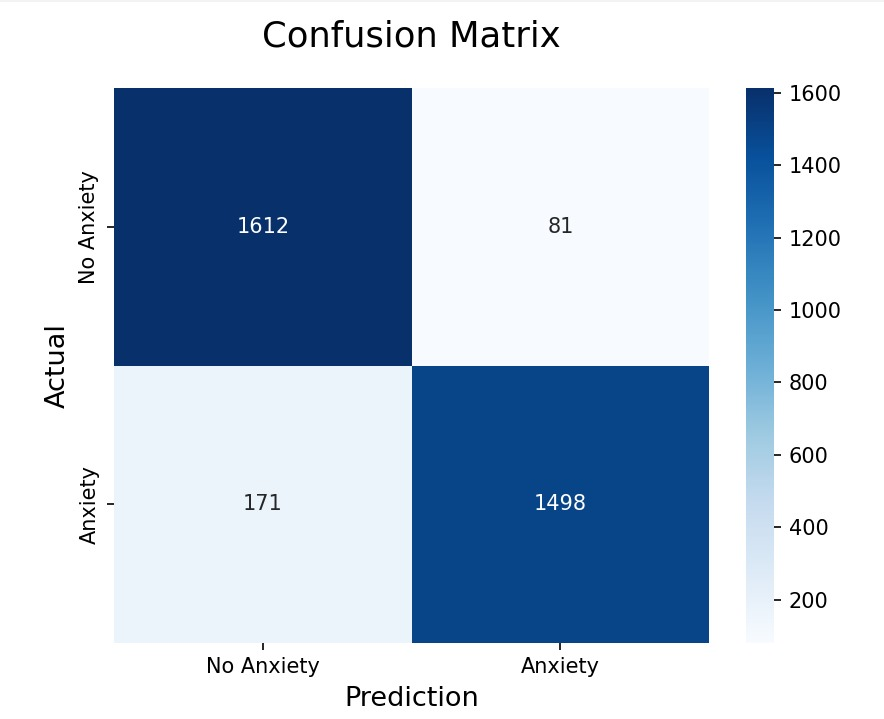
\includegraphics[width=0.9\textwidth]{Anxiety-Data-MLPClassifier.jpg}
\caption[Confusion matrix for anxiety data (Multi-layer Perceptron Classifier)]{\centering Confusion matrix for anxiety data using an Multi-layer Perceptron Classifier (large dataset). It shows 1612 true positives and 171 false positives for normal cases, and 1498 true positives with 81 false negatives for anxiety cases.}
\end{figure}

\vspace{0.5cm} % Add 1 cm of vertical space (adjust as needed)

\subsection{Depression Data}
\label{section:depressiondata}

\subsubsection{Linear Regression}
\label{section:regression}

\begin{itemize}
    \item \textbf{Hyperparameters:} ID, Text, Target
    \item \textbf{Target:} Normal (249), Depression (251)
    \item \textbf{Models:} Linear Regression with transformer Sentence Transformer with the data set encoding 'all-MiniLM-L6-v2'
    \item \textbf{Results:}
    \begin{itemize}
        \item \textbf{Accuracy:} 0.80
        \item \textbf{Average Precision:} 0.81
        \item \textbf{Precision for Depression Class:} 0.81
        \item \textbf{Precision for Normal Class:} 0.80
        \item \textbf{Recall for Depression Class:} 0.80
        \item \textbf{Recall for Normal Class:} 0.81
        \item \textbf{Confusion Matrix:}
    \end{itemize}
\end{itemize}

\begin{figure}[h]
\centering
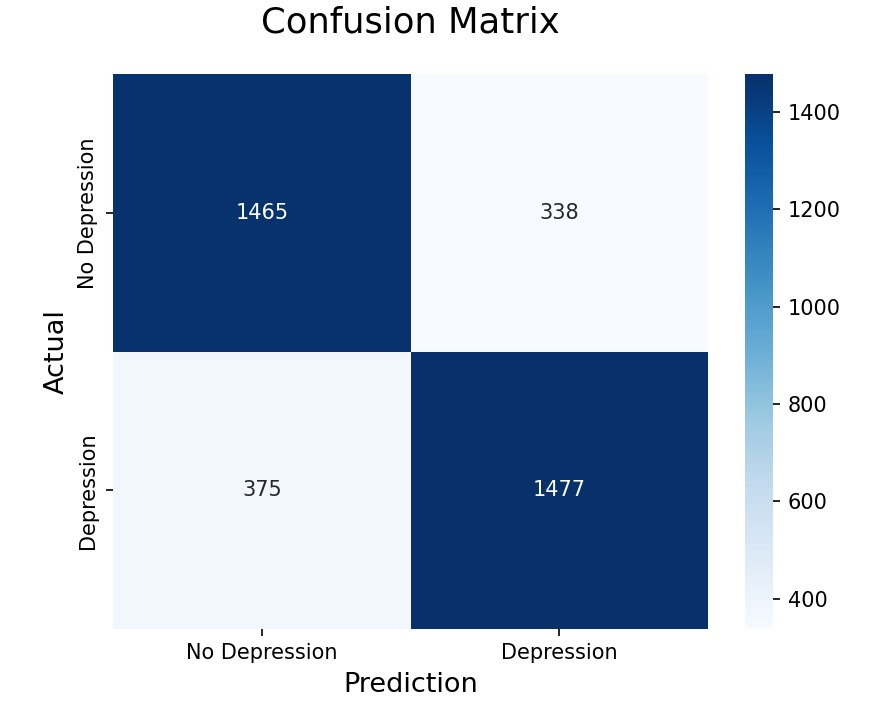
\includegraphics[width=0.9\textwidth]{Depression-Data-LinearRegression.jpg}
\caption[Confusion matrix for depression data (linear regression)]{\centering Confusion matrix for depression data using Linear Regression (large dataset). The results include 1465 true positives and 375 false positives for normal cases, as well as 1477 true positives and 338 false negatives for depression cases.}
\end{figure}

\vspace{0.5cm} % Add 1 cm of vertical space (adjust as needed)

\subsubsection{Decision Tree}
\label{section:tree}

\begin{itemize}
    \item \textbf{Hyperparameters:} ID, Text, Target
    \item \textbf{Target:} Normal (249), Depression (251)
    \item \textbf{Models:} Decision Tree with transformer Sentence Transformer with the data set encoding 'all-MiniLM-L6-v2'
    \item \textbf{Results:}
    \begin{itemize}
        \item \textbf{Accuracy:} 0.83
        \item \textbf{Average Precision:} 0.84
        \item \textbf{Precision for Depression Class:} 0.89
        \item \textbf{Precision for Normal Class:} 0.78
        \item \textbf{Recall for Depression Class:} 0.75
        \item \textbf{Recall for Normal Class:} 0.91
        \item \textbf{Confusion Matrix:}
    \end{itemize}
\end{itemize}

\begin{figure}[h]
\centering
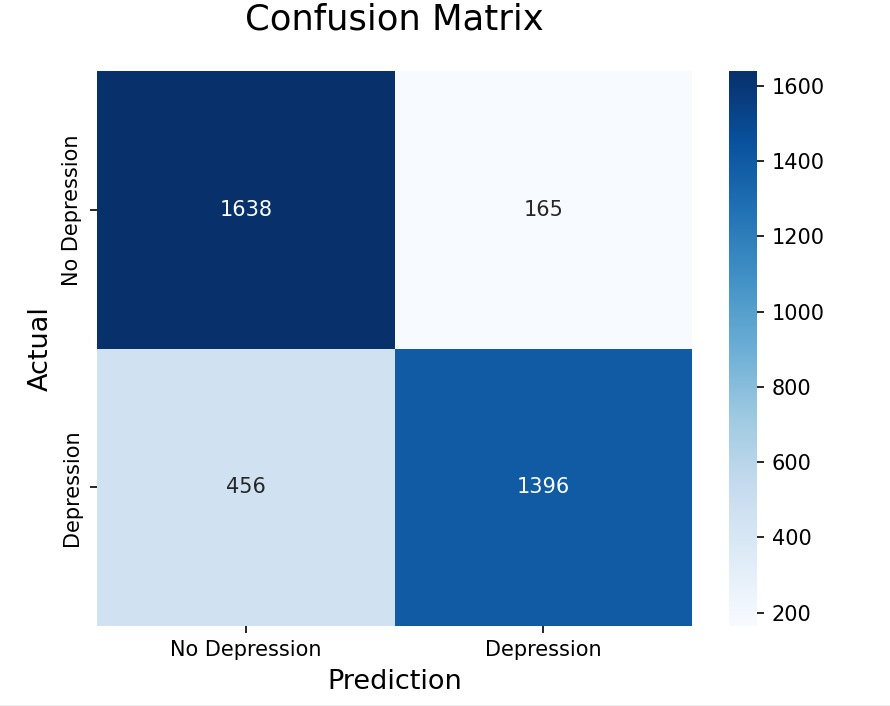
\includegraphics[width=0.9\textwidth]{Depression-Data-DecisionTree.jpg}
\caption[Confusion matrix for depression data (decision tree)]{\centering Confusion matrix for depression data using a Decision Tree (large dataset). It highlights 1638 true positives and 456 false positives for normal cases, with 1396 true positives and 165 false negatives for depression cases.}
\end{figure}

\vspace{0.5cm} % Add 1 cm of vertical space (adjust as needed)

\subsubsection{Multi-layer Perceptron Classifier}
\label{section:classifier}
\begin{itemize}
    \item \textbf{Hyperparameters:} ID, Text, Target
    \item \textbf{Target:} Normal (249), Depression (251)
    \item \textbf{Models:} Decision Tree with transformer Sentence Transformer with the data set encoding 'all-MiniLM-L6-v2'
    \item \textbf{Results:}
    \begin{itemize}
        \item \textbf{Accuracy:} 0.93
        \item \textbf{Average Precision:} 0.93
        \item \textbf{Precision for Depression Class:} 0.96
        \item \textbf{Precision for Normal Class:} 0.90
        \item \textbf{Recall for Depression Class:} 0.89
        \item \textbf{Recall for Normal Class:} 0.97
        \item \textbf{Confusion Matrix:}
    \end{itemize}
\end{itemize}

\begin{figure}[h]
\centering
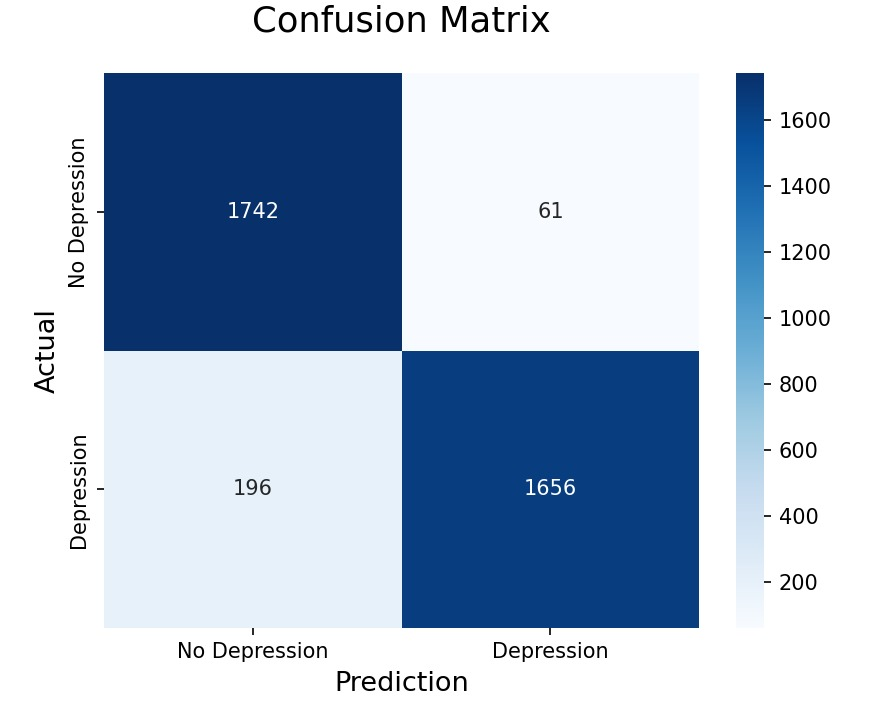
\includegraphics[width=0.9\textwidth]{Depression-Data-MLPClassifier.jpg}
\caption[Confusion matrix for depression data ( Multi-layer Perceptron Classifier)]{\centering Confusion matrix for depression data using an  Multi-layer Perceptron Classifier (large dataset). The matrix reports 1742 true positives and 196 false positives for normal cases, alongside 1656 true positives and 61 false negatives for depression cases.}
\end{figure}

\newpage
\begin{thebibliography}{99}

\bibitem{reddit_dataset} 
\textit{Reddit Mental Health Dataset}.  
Neel Ghoshal (2020).  
\\Available at: \url{https://www.kaggle.com/datasets/neelghoshal/reddit-mental-health-data}. 
\bibitem{emotion_dataset}  
\textit{Emotion Dataset}.  
Parul Pandey (2020).  
\\Available at: \url{https://www.kaggle.com/datasets/parulpandey/emotion-dataset/data?select=training.csv}.  

\end{thebibliography}






\end{document}